\documentclass[letter, 11pt, onesided]{memoir}

\usepackage[no-math]{fontspec}
\usepackage{xpatch}
	\renewcommand{\ttdefault}{ul9}
	\xpatchcmd{\ttfamily}{\selectfont}{\fontencoding{T1}\selectfont}{}{}
	\DeclareTextCommand{\nobreakspace}{T1}{\leavevmode\nobreak\ }
\usepackage{polyglossia} % English please
	\setdefaultlanguage[variant=us]{english}
\usepackage[charter,cal=cmcal]{mathdesign} %different font
\usepackage{avant}
\usepackage{microtype} % Less badboxes

\usepackage{calc, ifthen, xparse, xspace}
\usepackage{makeidx}
\usepackage[hidelinks]{hyperref}   % Internal hyperlinks
\usepackage{mathtools} % replaces amsmath
\usepackage{etoolbox}
\usepackage{bbm} %lower case blackboard font
\usepackage{amsthm, bm}
\usepackage{graphicx}
\usepackage{xcolor}
\usepackage{multicol}
\usepackage{tikz}
	\tikzset{>=latex}
	\usetikzlibrary{calc}
	\usetikzlibrary{backgrounds}
	\usetikzlibrary{patterns,decorations.pathreplacing}
	\usetikzlibrary{spy}
\usepackage{pgfplots}
	\pgfplotsset{compat=1.12}
	\usepgfplotslibrary{colormaps}
	\usepgfplotslibrary{patchplots}
	\usepgfplotslibrary{fillbetween}
\usepackage{tcolorbox}
	\tcbuselibrary{breakable}
\usepackage[inline,shortlabels]{enumitem}
\setlistdepth{9}

\usepackage{datatool}


\usepgfplotslibrary{external}
\tikzexternalize[prefix=tikz/]


%%% Specify the cool macros
\newcommand{\declarecommand}[1]{\providecommand{#1}{}\renewcommand{#1}}
\declarecommand{\R}{\mathbb{R}}  % we don't care if it's already defined.  We really want *this* command!
\declarecommand{\Z}{\mathbb{Z}}
\declarecommand{\Q}{\mathbb{Q}}
\declarecommand{\N}{\mathbb{N}}
\declarecommand{\C}{\mathbb{C}}
\declarecommand{\d}{\mathrm{d}}
\declarecommand{\dd}{\mathbbm{d}} % exterior derivative
\DeclareMathOperator{\Span}{span}
\DeclareMathOperator{\Img}{img}
\DeclareMathOperator{\Id}{id}
\DeclareMathOperator{\Range}{range}
\DeclareMathOperator{\Rref}{rref}
\DeclareMathOperator{\Rank}{rank}
\DeclareMathOperator{\Speed}{speed}
\DeclareMathOperator{\Vel}{velocity}
\DeclareMathOperator{\Accel}{accel}
\DeclareMathOperator{\Null}{null}
\DeclareMathOperator{\Nullity}{nullity}
\DeclareMathOperator{\Char}{char}
\DeclareMathOperator{\Proj}{proj}
\DeclareMathOperator{\Flux}{Flux}
\DeclareMathOperator{\Circ}{Circ}
\DeclareMathOperator{\Curl}{curl}
\DeclareMathOperator{\Dim}{dim}
\DeclareMathOperator{\Perp}{perp}
\DeclareMathOperator{\Ker}{kernel}
\DeclareMathOperator{\Trans}{\downarrow\!}
\DeclareMathOperator{\Transu}{\uparrow\!}
\DeclareMathOperator{\Arclen}{arc\,len}
\newcommand{\Arclenfrom}[3]{\Arclen #1 \Big|_{#2}^{#3}}
\newcommand{\proj}{\Proj}
\newcommand{\xhat}{{\hat {\mathbf x}}}
\newcommand{\yhat}{{\hat {\mathbf y}}}
\newcommand{\zhat}{{\hat {\mathbf z}}}
\newcommand{\mat}[1]{\begin{bmatrix*}[r]#1\end{bmatrix*}}
\newcommand{\matc}[1]{\begin{bmatrix}#1\end{bmatrix}}
\newcommand{\formarg}[2]{\big(#1;\, #2\big)}
\newcommand{\abs}[1]{\left\vert #1 \right\vert}
\newcommand{\norm}[1]{\left\| #1 \right\|}
\newcommand{\inner}[2]{\langle #1, #2 \rangle}
\newcommand{\set}[1]{\left\{ #1 \right\}}
% just to make sure it exists
\providecommand\given{}
% can be useful to refer to this outside \Set
\newcommand\SetSymbol[1][]{%
	\nonscript\::%
	\allowbreak
	\nonscript\:
	\mathopen{}}
\DeclarePairedDelimiterX\Set[1]\{\}{%
	\renewcommand\given{\SetSymbol[\delimsize]}
	#1
}
\renewcommand{\it}{\itshape}
% footnote without marker
\newcommand\blfootnote[1]{%
  \begingroup
  \renewcommand\thefootnote{}\footnote{#1}%
  \addtocounter{footnote}{-1}%
  \endgroup
}


% labels for source attributions
\NewDocumentCommand{\openstax}{o}{%
	\IfNoValueTF{#1}{%
		{\color{blue}\sffamily{OS}}%
	}{%
		{\color{blue}\sffamily{OS}}%  XXX Todo, make this href to the appropriate problem number
	}\xspace%
}

% labels for source attributions
\NewDocumentCommand{\grout}{o}{%
	\IfNoValueTF{#1}{%
		{\color{blue}\sffamily{G}}%
	}{%
		{\color{blue}\sffamily{G}}%  XXX Todo, make this href to the appropriate problem number
	}\xspace%
}

% set up some deep enumerate environments for the CC license
\newlist{ccEnumerate}{enumerate}{9}
\setlist[ccEnumerate,1]{label=\alph*.}
\setlist[ccEnumerate,2]{label=\arabic*.}
\setlist[ccEnumerate,3]{label=\Alph*.}
\setlist[ccEnumerate,4]{label=\roman*.}
\setlist[ccEnumerate,5]{label=(\alph*)}
\setlist[ccEnumerate,6]{label=(\arabic*)}
\setlist[ccEnumerate,7]{label=(\Roman*)}
\setlist[ccEnumerate,8]{label=(\Alph*)}
\setlist[ccEnumerate,9]{label=(\roman*)}


% other enumerate environments
\NewDocumentCommand{\prob}{o}{%
	\IfNoValueTF{#1}{%
		\refstepcounter{enumi}%
		\item[\theenumi]%
	}{%
		\refstepcounter{enumi}%
		\item[\theenumi \textsuperscript{#1}]%
	}%
}
\newenvironment{problist}{%
	\begin{enumerate}
	}{%
	\end{enumerate}
}
% an environment to store problem solutions
\newenvironment{solution}{%
		\par\color{blue} Solution: 
	}{%
		\ignorespacesafterend
}

%\newlist{problist}{enumerate}{3}
%\setlist[problist]{label=\arabic*}


%%% Specify the colors
\definecolor{myorange}{HTML}{F29B23}
\definecolor{myred}{HTML}{D13409}
\definecolor{mypink}{HTML}{B3094F}
\definecolor{mydark}{HTML}{23112A}
\definecolor{mygreen}{HTML}{34A320}
\definecolor{myblue}{HTML}{2F8CEF}

\colorlet{chapcolor}{myred}
\colorlet{seccolor}{myorange}
\colorlet{headertext}{myred!70!white}
\colorlet{ocre}{mypink}

%%% Specify custom fonts
%\newfontfamily{\sfreg}{Fira Sans}
%\newfontfamily{\firasans}
%  [Ligatures=TeX, % recommended
%   UprightFont={* Light},
%   ItalicFont={* Light Italic},
%   BoldFont={* Medium},
%   BoldItalicFont={* Medium Italic}]
%  {Fira Sans}



%%% PAGE LAYOUT
%%%------------------------------------------------------------------------------

\setlrmarginsandblock{0.15\paperwidth}{*}{1} % Left and right margin
\setulmarginsandblock{0.15\paperwidth}{*}{1}  % Upper and lower margin
\checkandfixthelayout

%%% SECTIONAL DIVISIONS
%%%------------------------------------------------------------------------------

%\maxsecnumdepth{subsection} % Subsections (and higher) are numbered
%\setsecnumdepth{subsection}
%
%\makeatletter %
%\makechapterstyle{standard}{
%  \setlength{\beforechapskip}{0\baselineskip}
%  \setlength{\midchapskip}{1\baselineskip}
%  \setlength{\afterchapskip}{8\baselineskip}
%  \renewcommand{\chapterheadstart}{\vspace*{\beforechapskip}}
%  \renewcommand{\chapnamefont}{\centering\normalfont\Large}
%  \renewcommand{\printchaptername}{\chapnamefont \@chapapp}
%  \renewcommand{\chapternamenum}{\space}
%  \renewcommand{\chapnumfont}{\normalfont\Large}
%  \renewcommand{\printchapternum}{\chapnumfont \thechapter}
%  \renewcommand{\afterchapternum}{\par\nobreak\vskip \midchapskip}
%  \renewcommand{\printchapternonum}{\vspace*{\midchapskip}\vspace*{5mm}}
%  \renewcommand{\chaptitlefont}{\centering\bfseries\LARGE}
%  \renewcommand{\printchaptertitle}[1]{\chaptitlefont ##1}
%  \renewcommand{\afterchaptertitle}{\par\nobreak\vskip \afterchapskip}
%}
%\makeatother
%
%\chapterstyle{standard}

%\setsecheadstyle{\normalfont\large\bfseries}
%\setsubsecheadstyle{\normalfont\normalsize\bfseries}
%\setparaheadstyle{\normalfont\normalsize\bfseries}
%\setparaindent{0pt}\setafterparaskip{0pt}

\renewcommand{\chapnumfont}{\normalfont\huge\sffamily\bfseries}
\renewcommand{\chaptitlefont}{\color{chapcolor}\chapnumfont\mdseries}
\renewcommand{\printchaptername}{\chapnumfont Chapter}
\makeatletter
	\renewcommand{\hangsecnum}{%
	  \def\@seccntformat##1{%
	    \makebox[0pt][r]{%
	      \color{seccolor}%
	      \csname the##1\endcsname
	      \quad
	    }%
	  }%
	}
\makeatother
%\setsecnumformat{\llap{\color{seccolor}\csname the#1\endcsname\quad}}

\setsecheadstyle{\Large\bfseries\sffamily\raggedright}
\setsubsecheadstyle{\large\sffamily\raggedright}
\setsubsubsecheadstyle{\normalsize\sffamily\raggedright}
\setsechook{\hangsecnum}
\setsubsechook{\defaultsecnum}
\setsubsubsechook{\defaultsecnum}


\makeatletter
	\setlength{\headwidth}{\textwidth}
	%\addtolength{\headwidth}{\marginparsep}
	%\addtolength{\headwidth}{\marginparwidth}
	\makepagestyle{serifpage}
	\makerunningwidth{serifpage}{\headwidth}
	\makeheadrule{serifpage}{\headwidth}{\normalrulethickness}
	\makeheadposition{serifpage}{flushright}{flushleft}{}{}
	\makepsmarks{serifpage}{%
		\let\@mkboth\markboth
		\def\chaptermark##1{\markboth{\textsf{\color{headertext}##1}}{\textsf{\color{headertext}##1}}}% % left & right marks
		\def\sectionmark##1{\markright{%
		\ifnum \c@secnumdepth>\z@
			{\color{seccolor}\sffamily\thesection\ }
		\fi
		\textsf{\color{headertext}##1}}}
	}
	\makeevenhead{serifpage}%
		{\normalfont\sffamily\thepage}{}{\normalfont\sffamily \leftmark}
	\makeoddhead{serifpage}%
		{\normalfont\sffamily \rightmark}{}{\normalfont\sffamily\thepage}
\makeatother

\pagestyle{serifpage}

%%% Theorem Environments

\makeatletter
	\newcommand{\intoo}[2]{\mathopen{]}#1\,;#2\mathclose{[}}
	\newcommand{\ud}{\mathop{\mathrm{{}d}}\mathopen{}}
	\newcommand{\intff}[2]{\mathopen{[}#1\,;#2\mathclose{]}}
	\newtheorem{notation}{Notation}[chapter]

	%%%%%%%%%%%%%%%%%%%%%%%%%%%%%%%%%%%%%%%%%%%%%%%%%%%%%%%%%%%%%%%%%%%%%%%%%%%
	%%%%%%%%%%%%%%%%%%%% dedicated to boxed/framed environements %%%%%%%%%%%%%%
	%%%%%%%%%%%%%%%%%%%%%%%%%%%%%%%%%%%%%%%%%%%%%%%%%%%%%%%%%%%%%%%%%%%%%%%%%%%
	\newtheoremstyle{orangenumbox}% % Theorem style name
	{0pt}% Space above
	{0pt}% Space below
	{\normalfont}% % Body font
	{}% Indent amount
	{\small\bfseries\sffamily\color{myorange}}% % Theorem head font
	{\;}% Punctuation after theorem head
	{0.25em}% Space after theorem head
	{\small\sffamily\color{myorange!80!black}\thmname{#1}\nobreakspace\thmnumber{\@ifnotempty{#1}{}\@upn{#2}}% Theorem text (e.g. Theorem 2.1)
	\thmnote{\nobreakspace\the\thm@notefont\sffamily\bfseries\color{black}---\nobreakspace#3.}} % Optional theorem note
	\renewcommand{\qedsymbol}{$\blacksquare$}% Optional qed square

	\newtheoremstyle{ocrenumbox}% % Theorem style name
	{0pt}% Space above
	{0pt}% Space below
	{\normalfont}% % Body font
	{}% Indent amount
	{\small\bfseries\sffamily\color{ocre}}% % Theorem head font
	{\;}% Punctuation after theorem head
	{0.25em}% Space after theorem head
	{\small\sffamily\color{ocre}\thmname{#1}\nobreakspace\thmnumber{\@ifnotempty{#1}{}\@upn{#2}}% Theorem text (e.g. Theorem 2.1)
	\thmnote{\nobreakspace\the\thm@notefont\sffamily\bfseries\color{black}---\nobreakspace#3.}} % Optional theorem note
	\renewcommand{\qedsymbol}{$\blacksquare$}% Optional qed square

	\newtheoremstyle{blacknumex}% Theorem style name
	{5pt}% Space above
	{5pt}% Space below
	{\normalfont}% Body font
	{} % Indent amount
	{\small\bfseries\sffamily}% Theorem head font
	{\;}% Punctuation after theorem head
	{0.25em}% Space after theorem head
	{\small\sffamily{\tiny\ensuremath{\blacksquare}}\nobreakspace\thmname{#1}\nobreakspace\thmnumber{\@ifnotempty{#1}{}\@upn{#2}}% Theorem text (e.g. Theorem 2.1)
	\thmnote{\nobreakspace\the\thm@notefont\sffamily\bfseries---\nobreakspace#3.}}% Optional theorem note

	\newtheoremstyle{blacknumbox} % Theorem style name
	{0pt}% Space above
	{0pt}% Space below
	{\normalfont}% Body font
	{}% Indent amount
	{\small\bfseries\sffamily}% Theorem head font
	{\;}% Punctuation after theorem head
	{0.25em}% Space after theorem head
	{\small\sffamily\thmname{#1}\nobreakspace\thmnumber{\@ifnotempty{#1}{}\@upn{#2}}% Theorem text (e.g. Theorem 2.1)
	\thmnote{\nobreakspace\the\thm@notefont\sffamily\bfseries---\nobreakspace#3.}}% Optional theorem note

	%%%%%%%%%%%%%%%%%%%%%%%%%%%%%%%%%%%%%%%%%%%%%%%%%%%%%%%%%%%%%%%%%%%%%%%%%%%
	%%%%%%%%%%%%% dedicated to non-boxed/non-framed environments %%%%%%%%%%%%%%
	%%%%%%%%%%%%%%%%%%%%%%%%%%%%%%%%%%%%%%%%%%%%%%%%%%%%%%%%%%%%%%%%%%%%%%%%%%%
	\newtheoremstyle{ocrenum}% % Theorem style name
	{5pt}% Space above
	{5pt}% Space below
	{\normalfont}% % Body font
	{}% Indent amount
	{\small\bfseries\sffamily\color{ocre}}% % Theorem head font
	{\;}% Punctuation after theorem head
	{0.25em}% Space after theorem head
	{\small\sffamily\color{ocre}\thmname{#1}\nobreakspace\thmnumber{\@ifnotempty{#1}{}\@upn{#2}}% Theorem text (e.g. Theorem 2.1)
	\thmnote{\nobreakspace\the\thm@notefont\sffamily\bfseries\color{black}---\nobreakspace#3.}} % Optional theorem note
	\renewcommand{\qedsymbol}{$\blacksquare$}% Optional qed square

    \newtheoremstyle{bluenum}% % Theorem style name
	{5pt}% Space above
	{5pt}% Space below
	{\normalfont}% % Body font
	{}% Indent amount
	{\small\bfseries\sffamily\color{myblue}}% % Theorem head font
	{\;}% Punctuation after theorem head
	{0.25em}% Space after theorem head
	{\small\sffamily\color{myblue}\thmname{#1}\nobreakspace\thmnumber{\@ifnotempty{#1}{}\@upn{#2}}% Theorem text (e.g. Theorem 2.1)
	\thmnote{\nobreakspace\the\thm@notefont\sffamily\bfseries\color{black}---\nobreakspace#3.}} % Optional theorem note
	\renewcommand{\qedsymbol}{$\blacksquare$}% Optional qed square

    \newtheoremstyle{greennum}% % Theorem style name
	{5pt}% Space above
	{5pt}% Space below
	{\normalfont}% % Body font
	{}% Indent amount
	{\small\bfseries\sffamily\color{mygreen}}% % Theorem head font
	{\;}% Punctuation after theorem head
	{0.25em}% Space after theorem head
	{\small\sffamily\color{mygreen}\thmname{#1}\nobreakspace\thmnumber{\@ifnotempty{#1}{}\@upn{#2}}% Theorem text (e.g. Theorem 2.1)
	\thmnote{\nobreakspace\the\thm@notefont\sffamily\bfseries\color{black}---\nobreakspace#3.}} % Optional theorem note
	\renewcommand{\qedsymbol}{$\blacksquare$}% Optional qed square
	\makeatother

	% Defines the theorem text style for each type of theorem to one of the three styles above
	\newcounter{dummy}
	\numberwithin{dummy}{section}
	\theoremstyle{orangenumbox}
	\newtheorem{theoremeT}[dummy]{Theorem}
	\theoremstyle{ocrenumbox}
	\newtheorem{problem}{Problem}[chapter]
	\newtheorem{exerciseT}{Exercise}[chapter]
	\theoremstyle{blacknumex}
	\newtheorem{exampleT}{Example}[chapter]
	\theoremstyle{blacknumbox}
	\newtheorem{vocabulary}{Vocabulary}[chapter]
	\newtheorem{definitionT}{Definition}[section]
	\newtheorem{corollaryT}[dummy]{Corollary}
	\theoremstyle{bluenum}
	\newtheorem{propositionT}[dummy]{Proposition}
    \theoremstyle{greennum}
    \newtheorem*{proofT}{Proof}

	%----------------------------------------------------------------------------------------
	%	DEFINITION OF COLORED BOXES
	%----------------------------------------------------------------------------------------

	\RequirePackage[framemethod=default]{mdframed} % Required for creating the theorem, definition, exercise and corollary boxes

	% Theorem box
	\newmdenv[skipabove=7pt,
	skipbelow=7pt,
	rightline=false,
	leftline=true,
	topline=false,
	bottomline=false,
	backgroundcolor=myorange!20,
	linecolor=myorange,
	innerleftmargin=5pt,
	innerrightmargin=5pt,
	innertopmargin=5pt,
	innerbottommargin=5pt,
	leftmargin=0cm,
	rightmargin=0cm,
	linewidth=4pt]{tBox}

	% Exercise box
	\newmdenv[skipabove=7pt,
	skipbelow=7pt,
	rightline=false,
	leftline=true,
	topline=false,
	bottomline=false,
	backgroundcolor=ocre!10,
	linecolor=ocre,
	innerleftmargin=5pt,
	innerrightmargin=5pt,
	innertopmargin=5pt,
	innerbottommargin=5pt,
	leftmargin=0cm,
	rightmargin=0cm,
	linewidth=4pt]{eBox}

	% Definition box
	\newmdenv[skipabove=7pt,
	skipbelow=7pt,
	rightline=false,
	leftline=true,
	topline=false,
	bottomline=false,
	linecolor=ocre,
	innerleftmargin=5pt,
	innerrightmargin=5pt,
	innertopmargin=0pt,
	leftmargin=0cm,
	rightmargin=0cm,
	linewidth=4pt,
	innerbottommargin=0pt]{dBox}

	% Corollary box
	\newmdenv[skipabove=7pt,
	skipbelow=7pt,
	rightline=false,
	leftline=true,
	topline=false,
	bottomline=false,
	linecolor=gray,
	backgroundcolor=black!5,
	innerleftmargin=5pt,
	innerrightmargin=5pt,
	innertopmargin=5pt,
	leftmargin=0cm,
	rightmargin=0cm,
	linewidth=4pt,
	innerbottommargin=5pt]{cBox}

	% Exercises box
	\newmdenv[skipabove=7pt,
	skipbelow=7pt,
	rightline=false,
	leftline=false,
	topline=false,
	bottomline=false,
	linecolor=gray,
	backgroundcolor=blue!5,
	innerleftmargin=5pt,
	innerrightmargin=18pt,
	innertopmargin=0pt,
	innerbottommargin=6pt,
	leftmargin=0cm,
	rightmargin=0cm,
	linewidth=4pt]{exsBox}

    % Propositions box
    \newmdenv[skipabove=7pt,
	skipbelow=7pt,
	rightline=false,
	leftline=true,
	topline=false,
	bottomline=false,
	backgroundcolor=myblue!20,
	linecolor=myblue,
	innerleftmargin=5pt,
	innerrightmargin=5pt,
	innertopmargin=0pt,
	innerbottommargin=5pt,
	leftmargin=0cm,
	rightmargin=0cm,
	linewidth=4pt]{pBox}

    % Proof box (not a real box)
    \newmdenv[skipabove=7pt,
	skipbelow=7pt,
	rightline=false,
	leftline=true,
	topline=false,
	bottomline=false,
	backgroundcolor=white,
	linecolor=mygreen,
	innerleftmargin=5pt,
	innerrightmargin=5pt,
	innertopmargin=0pt,
	innerbottommargin=5pt,
	leftmargin=0cm,
	rightmargin=0cm,
	linewidth=4pt]{pfBox}

\makeatother

% Creates an environment for each type of theorem and assigns it a theorem text style from the "Theorem Styles" section above and a colored box from above
\newenvironment{theorem}{\begin{tBox}\begin{theoremeT}}{\end{theoremeT}\end{tBox}}
\renewenvironment{proof}{\begin{pfBox}\begin{proofT}}{\end{proofT}\end{pfBox}}
\newenvironment{exercise}{\begin{eBox}\begin{exerciseT}}{\end{exerciseT}\end{eBox}}
%\newenvironment{exercise}{\begin{eBox}\begin{exerciseT}}{\hfill{\color{ocre}\tiny\ensuremath{\blacksquare}}\end{exerciseT}\end{eBox}}
\newenvironment{definition}{\begin{dBox}\begin{definitionT}}{\end{definitionT}\end{dBox}}
\newenvironment{example}{\begin{exampleT}}{\hfill{\tiny\ensuremath{\blacksquare}}\end{exampleT}}
\newenvironment{corollary}{\begin{cBox}\begin{corollaryT}}{\end{corollaryT}\end{cBox}}
\newenvironment{proposition}{\begin{pBox}\begin{propositionT}}{\end{propositionT}\end{pBox}}

\newenvironment{exercises}{%
	\begin{multicols*}{2}[\begin{exsBox}{\subsection*{Exercises for \thesection}}\vspace{-0pt}\end{exsBox}]\small %
	}{%
	\end{multicols*}%
	\clearpage
}
\newenvironment{answer}{\begin{quote}}{\end{quote}}


%%% THE DOCUMENT
%%% Where all the important stuff is included!
%%%-----------------------------------------------------------------------------------------------------
\author{Bailey Bjornstad}
\title{Math 321: MENU Real Analysis}

\renewcommand{\maketitlehooka}{\color{chapcolor}\chapnumfont\Huge}
\renewcommand{\maketitlehookb}{\color{black}\normalfont}
\renewcommand{\maketitlehookc}{\small
	\begin{center}
		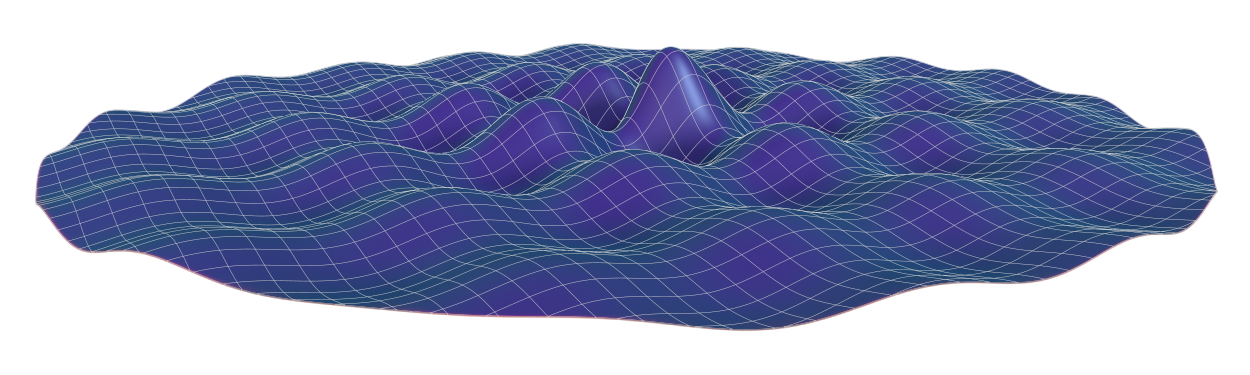
\includegraphics[width=6in]{resources/cover-render-lines-lowres.png}
	\end{center}
}
\renewcommand{\maketitlehookd}{
	\begin{center}
		
\includegraphics[width=1in]{resources/doclicense-CC-by-sa.pdf}
	\end{center}
}
\usepackage{lipsum} % Just to put in some text

\begin{document}

\frontmatter
\begin{titlingpage}
    \calccentering{\unitlength}
    \begin{adjustwidth*}{\unitlength}{-\unitlength}
        \maketitle
    \end{adjustwidth*}
\end{titlingpage}

\tableofcontents*
\clearpage


\mainmatter
\chapter{Measure Theory and Lebesgue Integration}
    \section{The Integral, Generally}

Here, we would like to explore a few basic properties that we want any integral to have, whether it be
the more familiar Riemann-Stieltjes integral or the Lebesgue integral that we will be developing here.
However, to consider these basic properties, we must have a space of functions that we can integrate!
Though we will develop more rigorous properties of these function spaces later on, for now we will
simply assume that we have a vector space $\mathcal{V}$ of either real or complex-valued functions that
are integrable. Then, we might want our integral to satisfy the following properties.
\begin{enumerate}
    \item   \emph{Linearity.} Given two functions $f$ and $g$ in $\mathcal{V}$ and scalars (either
        real or complex) $a$ and $b$, then
        \[
            \int (a f + b g)\,\d x = a \int f\,\d x + b \int g\,\d x.  
        \]
    \item   \emph{Monotonicity.} This property can only hold in the real-valued case, as we require an
        order to consider monotonicity. However, if $f(x) \geq g(x)$ for all $x$, then
        \[
            \int f \,\d x \geq \int g \,\d x.  
        \]
    \item   \emph{Additivity.}
        \[
            \int_a^b f\,\d x + \int_b^c f\,\d x = \int_a^c f\,\d x.  
        \]
    \item   \emph{Constant Functions.} Suppose that $f(x) = c$ for some scalar $c$. Then
        \[
            \int_a^b f\,\d x = c(b-a).  
        \]
    \item   \emph{Small Sets.} For the moment, this will essentially mean finite. We will continue to
        develop exactly what is meant by a ``small set'' during our discussion of measure theory.
        However, if $f(x) = g(x)$ except on a small set (e.g. finite) then
        \[
            \int f\,\d x = \int g\,\d x.  
        \]
\end{enumerate}

From here, we are able to prove a few basic propositions about any integral that satisfies the above
properties.
\begin{proposition}
    Given an integral that satisfies properties 1-5 from above, then
    \[
        \abs{\int f\,\d x} \leq \int \abs{f}\,\d x.
    \]
\end{proposition}
\begin{proof}
    Note that for any $x$, $\abs{f(x)} \geq f(x)$. Then, by monotonicity we have that
    \[
        \int f \,\d x \leq \int \abs{f} \,\d x.
    \]
    Further, we also know that for any $x$, $\abs{f(x)} \geq -f(x)$. A second application of
    monotonicity thus shows that
    \[
        \int -f \,\d x \leq \int \abs{f} \,\d x.  
    \]
    By linearity, we then have that both
    \[
        -\int f\,\d x \leq \int \abs{f} \,\d x \quad \int f\,\d x \leq \int \abs{f}\,\d x.
    \]
    This clearly shows the claim.
\end{proof}

However, we still lack a good conception of what exactly it means for a function to be integrable. How
do we know when these integrals should exist? In order to develop what it means for a function to be
integrable, we must first know about an important class of functions known as step functions.
\begin{definition}
    A function $s$ is a step function if there exists a finite set of points $\set{0 = x_0, x_1, x_2,
    \cdots, x_n = 1}$ so that on each $(x_{i-1}, x_i)$, $s(x)$ is constant. We will let $\mathcal{S}$
    denote the set of all step functions defined on $[0,1]$.
\end{definition}



\section{Endomorphisms on Hilbert Spaces}
Here we will consider a special class of functions defined on general Hilbert spaces: the endomorphims.
\begin{definition}
    If $\mathcal{H}$ is a Hilbert space, then a function $f: \mathcal{H} \to \mathcal{H}$ is an
    \emph{endomorphism} if it is linear and continuous.
\end{definition}
We will now show an important result that is useful in characterizing functions as endomorphisms,
although it has further applications beyond this.
\begin{proposition}
    A linear function $f: \mathcal{H}_1 \to \mathcal{H}_2$, where $\mathcal{H}_1$ and $\mathcal{H}_2$ are
    Hilbert spaces, is continuous if and only if it is bounded.
\end{proposition}
\begin{proof}
    We will begin by showing that a bounded linear function $f$ is continuous. To this end, note that
    for every $x \in \mathcal{H}_1$ that $\norm{f(x)} \leq M\norm{x}$, by assumption of boundedness.
    Therefore, given $\epsilon > 0$, put $\delta = \epsilon / M$. Then, if $\norm{x-y} < \delta$ when
    $x, y \in \mathcal{H}_1$, then $\norm{f(x) - f(y)} = \norm{f(x-y)} \leq M\norm{x-y} < \epsilon$.
    This shows that $f$ is continuous.

    We wiill next show that a continous linear function is bounded. By the assumption of continuity,
    there must exist some $\delta > 0$ so that if $\norm{y} < \delta$ then $\norm{f(y)} < 1$ for $y \in
    \mathcal{H}_1$. Then, for an arbitrary $x \in \mathcal{H}$, we have that
    \[
        \norm{f(x)} = \norm{f\left( \frac{\norm{x}}{\delta} \frac{\delta}{\norm{x}} x \right)} =
        \norm{\frac{\norm{x}}{\delta} f\left( \delta \frac{x}{\norm{x}} \right)} = \frac{1}{\delta}
        \norm{f\left(\delta \frac{x}{\norm{x}}\right)} < \frac{1}{\delta}.
    \]
    This shows that $f$ is then bounded.
\end{proof}

As an aside, the previous proposition actually holds for any normed vector spaces, and does not require
that $\mathcal{H}_1$ and $\mathcal{H}_2$ are Hilbert spaces. However, we will nearly always be
considering functions on Hilbert spaces. In fact, we even have special notation for the set of
endomorphisms of a Hilbert space.
\begin{definition}
    If $\mathcal{H}$ is a Hilbert space, we define $\mathscr{E}(\mathcal{H}) = \set{f: \mathcal{H} \to
    \mathcal{H} \mid f \text{ is linear and continuous}}$. We may equip the set
    $\mathscr{E}(\mathcal{H})$ with a norm defined by
    \[
        \norm{A} = \sup \set{\norm{Ax} \mid x \in \mathcal{H} \text{ and } \norm{x} = 1}.
    \]
    We call this norm the \emph{operator norm} of $A$.
\end{definition}
With this new definition, we can begin to explore some properties of the endomorphisms of a Hilbert
space. But first, we should check to make sure that the operator norm is a good norm.
\begin{proposition}
    If $\mathcal{H}$ is a Hilbert space, then the operator norm of $\mathscr{E}(\mathcal{H})$ is a good
    norm. This is to say that given $A \in \mathscr{E}(\mathcal{H})$, the operator norm satisfies that
    \begin{enumerate}
        \item   $\norm{A} \geq 0$.
        \item   $\norm{A} = 0$ if and only if $A$ is identically $0$.
        \item   $\norm{cA} = \abs{c}\norm{A}$
        \item   $\norm{A + B} \leq \norm{A} + \norm{B}$.
    \end{enumerate}
\end{proposition}
\begin{proof}
    We will show each property of the norm separately.
    \begin{enumerate}
        \item   Note that $\norm{A} = \sup_{\norm{x} = 1} \norm{Ax}$. By the definition of the Hilbert
            space norm, we then have that $\norm{A} = \sup_{\norm{x} = 1} \sqrt{\abs{\inner{Ax}{Ax}}^2}
            \geq 0$ always.
        \item   Suppose first that $A$ is identically $0$. Then, for any $x \in H$ we have that $Ax =
            0$, so that $\norm{Ax} = 0$. Therefore, we also have that $\norm{A} = \sup_{\norm{x} = 1}
            \norm{Ax} = 0$. Next suppose that $\norm{A} = 0$. Then we have that $\sup_{\norm{x} = 1}
            \norm{Ax} = 0$. Thus, for any $x$ with $\norm{x} = 1$, we have that $\norm{Ax} \leq 0$.
            However, by properties of the Hilbert space norm, we also have that $\norm{Ax} \geq 0$. This
            shows that $\norm{Ax} = 0$ for any $x$ with $\norm{x} = 1$. This is only true if $A$ is
            identically $0$.
        \item   Let $c$ be a scalar. Then, we have that $\norm{cA} = \sup_{\norm{x} = 1} \norm{cAx} =
            \sup_{\norm{x} = 1} \abs{c}\norm{Ax} = \abs{c} \norm{A}$.
        \item   Let $B \in \mathscr{E}(\mathcal{H})$ be arbitrary. Then, $\norm{A + B} = \sup_{\norm{x}
            = 1} \norm{(A+B)(x)} = \sup_{\norm{x} = 1} \norm{Ax + Bx}$. By the triangle inequality of
            the Hilbert space norm, we then have that $\norm{A + B} \leq \sup_{\norm{x} = 1} (\norm{Ax}
            + \norm{Bx}) = \norm{A} + \norm{B}$. We are justified in splitting up the supremum over the
            sum since both $\sup_{\norm{x} = 1} \norm{Ax}$ and $\sup_{\norm{x} = 1} \norm{Bx}$ are well
            defined.
    \end{enumerate}
    This shows that the operator norm is a good norm.
\end{proof}

We have established that the operator norm is a good norm, but we also have two more useful properties
of the operator norm.
\begin{proposition}
    Given $A \in \mathscr{E}(\mathcal{H})$,
    \begin{enumerate}
        \item   $\norm{Ax} \leq \norm{A} \norm{x}$,
        \item   $\norm{AB} \leq \norm{A}\norm{B}$.
    \end{enumerate}
\end{proposition}
\begin{proof}
    First, for any $y \in \mathcal{H}$ with $\norm{y} = 1$, we have that $\norm{Ay} \leq \norm{A}$ by
    the definition of the operator norm. Therefore, given an arbitrary $x \in \mathcal{H}$, we have that
    \[
        \norm{Ax} = \norm{A\left(\norm{x} \frac{x}{\norm{x}}\right)} = \norm{x}
        \norm{A\left(\frac{x}{\norm{x}}\right)}.  
    \]
    Then, since $x/\norm{x}$ is a unit vector, we find that $\norm{Ax} \leq \norm{A}\norm{x}$. Thus,
    given $B \in \mathcal{H}$, we then have that $\norm{AB(x)} \leq \norm{A}\norm{Bx} \leq
    \norm{A}\norm{B}\norm{x}$.
\end{proof}

Now, equipped with a series of properties about the operator norm, we are prepared to tackle an
important and highly consequential fact about the endomorphisms of a Hilbert space.
\begin{theorem}
    Given $\mathcal{H}$ a Hilbert space, $\mathscr{E}(\mathcal{H})$ equipped with the operator norm is a
    complete metric space.
\end{theorem}
\begin{proof}
    Recall that a metric space $X$ is complete if every Cauchy sequence in $X$ converges to a point in
    $X$. Thus, since the operator norm is a good norm, it defines a metric $d: \mathscr{E}(\mathcal{H})
    \to \R$ by $d(A,B) = \norm{A-B}$. Thus, to show that $\mathscr{E}(\mathcal{H})$ is complete, we need
    to show that Cauchy sequences converge.

    Suppose that $\set{A_n}$ is a Cauchy sequence in $\mathscr{E}(\mathcal{H})$. This is to say that
    given $\epsilon > 0$, there exists some $N \in \N$ so that $n, m \geq N$ implies that $\norm{A_n -
    A_m} < \epsilon$. Further, for a fixed $x \in \mathcal{H}$, it is clear that the sequence
    $\set{A_nx}$ is a Cauchy sequence in $\mathcal{H}$. Since $\mathcal{H}$ is a Hilbert space and is
    thus complete, then
    \[
        Ax = \lim_{n \to \infty} A_nx
    \]
    exists. We claim that $A$ is the limit of the Cauchy sequence $\set{A_n}$, or equivalently that
    \[
        \lim_{n \to \infty} \norm{A - A_n} = 0.  
    \]
    In particular, we have that
    \begin{align*}
        \norm{A_nx - Ax} &= \lim_{m \to \infty} \norm{A_n x - A_m x}\\
                         &\leq \limsup_{m \to \infty} \norm{A_n - A_m} \norm{x} \\
                         &< \epsilon \norm{x}
    \end{align*}
    if $n,m \geq N$. Therefore, we now take the $\sup$ over all $x \in \mathcal{H}$ with $\norm{x} = 1$.
    This shows that
    \begin{align*}
        \norm{A_n - A} &= \sup_{\norm{x} = 1} \norm{(A_n - A)(x)} \\
                       &\leq \sup_{\norm{x} = 1} \epsilon\norm{x} = \epsilon.
    \end{align*}
    Thus, if $n \geq N$, we find that $\norm{A_n - A} \leq \epsilon$, which thus shows that $\lim_{n \to
    \infty} \norm{A_n - A} = 0$. Therefore, $\lim_{n \to \infty} A_n = A$ under the operator norm. This
    shows that $\mathscr{E}(\mathcal{H})$ is complete.
\end{proof}

We will now take a small digression into the realm of Functional Analysis to briefly discuss an
important consequence of the following theorem.
\begin{theorem}[The Open Mapping Theorem]
    Begin by defining 
    \[
        B_{\mathcal{H}}(r) = \set{x \in \mathcal{H} \mid \norm{x} < r}.
    \]
    Then, if $A:
    \mathcal{H}_1 \to \mathcal{H}_2$ is a bounded linear isomorphism (i.e.  that $A$ is a bijection,
    bounded, and linear), there exists some $r > 0$ so that
    \[
        B_{\mathcal{H}_2}(r) \subset A(B_{\mathcal{H}_1}(1)).
    \]
\end{theorem}
The details of the proof are outside the scope of this course, and so we will not present them here.
Instead, we will prove an important corollary of the Open Mapping Theorem.
\begin{proposition}
    If $A: \mathcal{H} \to \mathcal{H}$ is bounded, linear, and has a well defined algebraic inverse
    $A^{-1}: \mathcal{H} \to \mathcal{H}$, then $A^{-1}$ is bounded.
\end{proposition}
\begin{proof}
    By the Open Mapping Theorem, $A(B(1)) \supset B(r) \supset \overline{B(r/2)}$, for some $r$ (note
    that $B(r) = \set{x \in \mathcal{H} \mid \norm{x} < r}$). Let $S = \set{x \mid \norm{x} = r/2}$.
    Note that $S \subset A(B(1))$. Then, if $y \in S$, we have that $y = Ax$ for some $x$ with $\norm{x}
    \leq 1$. This is to say that $x = A^{-1} y$, so that 
    \[
        1 \geq \norm{x} = \norm{A^{-1} y}
    \]
    wait no something is very wrong here.
\end{proof}

    \clearpage



\end{document}
